
\section{Aleatoriedad y procesos estocásticos}

\subsection{Desigualdad de Jensen}
Sea la función convexa $f(S)$ (que se curva hacia arriba, con forma de cuenco) de la variable aleatoria $S$, entonces
\[\mathbb{E}[f(S)] \geq f(\mathbb{E}[S])\]
De hecho, la diferencia es de
\[\frac{1}{2}f''(\mathbb{E}[S])\mathbb{E}[\epsilon]\]
donde $\epsilon$ es la desviación de $S$ de la media, i.e $S=\mathbb{E}[S]+\epsilon$.


\subsection{Propiedad de Markov}
\textit{El futuro depende solo del presente, no del pasado.} Se usa en los caminos aleatorios para decir que el valor $S_t+1$ solo depende de $S_t$, es decir,
\[\mathbb{P}(X_{t+s} \in A \mid X_t = x, X_{t_1} = x_1, \ldots, X_{t_n} = x_n) 
= \mathbb{P}(X_{t+s} \in A \mid X_t = x)\]



\subsection{Propiedad de martingala}
\textit{Lo que esperas tener en el futuro, sabiendo todo hasta ahora, es exactamente lo que tienes ahora}. Es decir, el valor esperado de algo en un juego justo es exactamente lo que tienes ahora:
\[\mathbb{E}[S_i|S_j, j<i]=S_j\]



\subsection{Lema de Itô}
Sea
\[dS = a(S,t)dt + b(S,t)d\mathnormal{X}\]
entonces
\begin{equation}
    \boxed{dV = \left( \frac{dV}{dt} +  a\frac{dV}{dS} + \frac{1}{2}b^2\frac{d^2V}{dS^2} \right)dt + b\frac{dV}{dS}d\mathnormal{X}}
\end{equation}\label{Ito}
En el apéndice~\ref{CalcIto} se encuentra la fórmula para dimensiones mayores.

\subsection{Algunos ejemplos de caminos aleatorios}

\begin{itemize}
    \item \textbf{Brownian Motion with Drift}: $\boxed{dS = \mu dt + \sigma d\mathnormal{X}}$
    \begin{figure}[H]
        \centering
        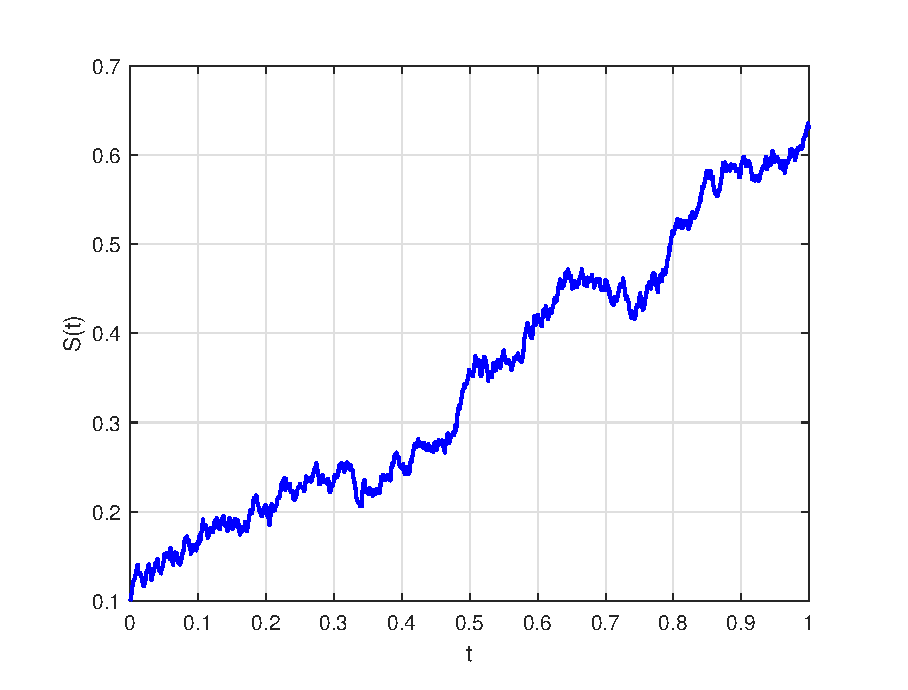
\includegraphics[width=0.65\linewidth]{Imagenes/3_Aleatoriedad/BrownianMotionDrift.eps}
        \caption{Brownian Motion with Drift}
    \end{figure}
    \item \textbf{The Lognormal Random Walk}: $\boxed{dS = S\mu dt + S\sigma d\mathnormal{X}}$
    \begin{figure}[H]
        \centering
        \includegraphics[width=0.65\linewidth]{Imagenes/3_Aleatoriedad/LognormalRandomWalk.eps}
        \caption{The Lognormal Random Walk}
    \end{figure}
    \item \textbf{A Mean-reverting Random Walk}: reversion a la media, cuando se esta fuera del crecimiento normal el camino tiende a corregirse.\\
    Su EDE es 
    \[
        \boxed{dS = \kappa(\theta+S) dt + \sigma d\mathnormal{X}}
    \]
    donde $\kappa$ es la velocidad de reversión a la media, $\theta$ es la tasa de interés a largo plazo y $\sigma$ es la volatilidad. Un ejemplo común es el modelo Vasicek para el ratio de interés, $dr = \kappa(\theta+r) dt + \sigma d\mathnormal{X}$
    \begin{figure}[H]
        \centering
        \includegraphics[width=0.65\linewidth]{Imagenes/3_Aleatoriedad/MeanRevertingWalk.eps}
        \caption{Mean-reverting Random Walk}
    \end{figure}
\end{itemize}



\subsection{Función de densidad de transición}
Es la \textit{`probabilidad de que una variable aleatoria $y$ esté entre $a$ y $b$ en el instante futuro $t'$, sabiendo que ha empezado con un valor $y$ en el instante $t$`}. En concreto la función de densidad de transición $p(y, t; y', t')$ es:
\[
    \boxed{\text{Prob}(a<y'<b\text{ en }t' | y\text{ en }t) = \int_a^b p(y, t; y', t') dy'}
\]

\subsubsection{Ecuación de Fokker-Planck o de Kolmogorov hacia delante}
Se centra en cómo evoluciona la transición con respecto al tiempo futuro $t'$. Se enfoca en el destino del proceso y cómo cambia la probabilidad de estar en distintos valores futuros $y'$ a medida que avanza el tiempo $t'$. Sabiendo que la variable aleatoria cumple la EDE
\[
    dy = A(y, t) dt + B(y, t) d\mathnormal{X}
\]
entonces la función de densidad de transición es la solución de la ecuación diferencial parcial
\[
    \boxed{\frac{\partial p}{\partial t'} = \frac{1}{2} \frac{\partial^2}{\partial y'^2} \left( B(y', t')^2 p \right) - \frac{\partial}{\partial y'} \left( A(y', t') p \right)}
\]
por ejemplo para la EDE
\[
    dS = \mu S dt + \sigma S d\mathnormal{X}
\]
se tiene que reolver la EDP
\[
    \frac{\partial p}{\partial t'} = \frac{1}{2} \frac{\partial^2}{\partial S'^2} \left( \sigma^2 S'^2 p \right) - \frac{\partial}{\partial S'} \left( \mu S' p \right)
\]
que da como solución
\[
    p(S, t; S', t') = \frac{1}{\sigma S' \sqrt{2\pi (t'-t)}} \exp\left( -\frac{ \left( \log(S/S') + (\mu - \frac{1}{2}\sigma^2)(t'-t) \right)^2 }{ 2\sigma^2 (t'-t) } \right)
\]
\begin{figure}[H]
    \centering
    \begin{subfigure}[b]{0.45\linewidth}
        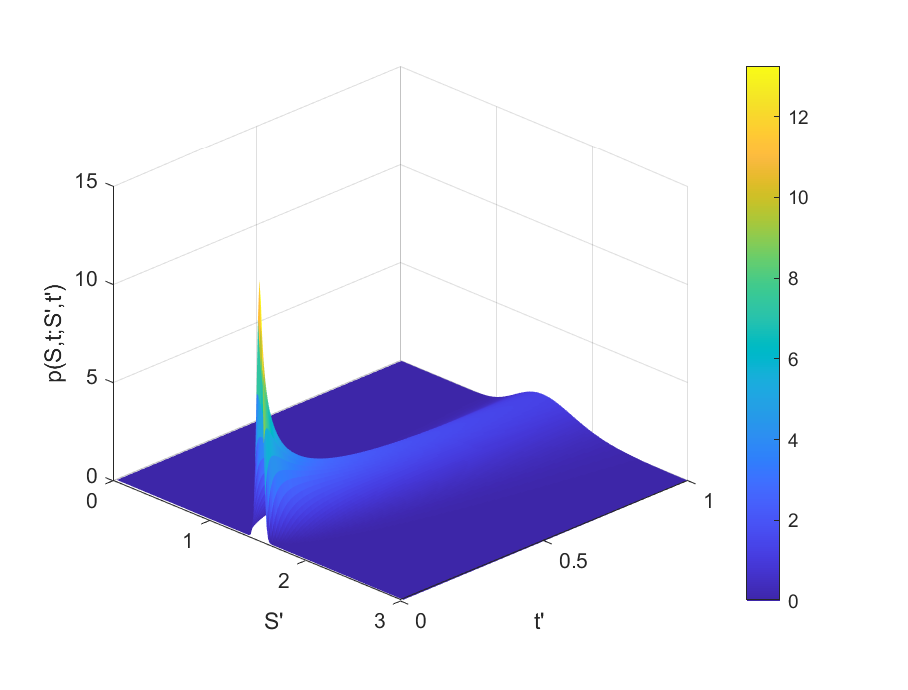
\includegraphics[width=\linewidth]{Imagenes/3_Aleatoriedad/PDF_3D.eps}
    \end{subfigure}
        \begin{subfigure}[b]{0.45\linewidth}
        \includegraphics[width=\linewidth]{Imagenes/3_Aleatoriedad/PDF_2D.eps}
    \end{subfigure}
    \caption{Función de densidad de transición}
\end{figure}



\subsubsection{Ecuación de Kolmogorov hacia detrás}
Se centra en cómo evoluciona la densidad de transición con respecto al tiempo actual $t$. Se enfoca más en el origen  y cómo cambian las probabilidades de llegar al punto $y'$, $t'$ dependiendo de donde se está en el momento. La EDP es
\[
    \boxed{\frac{\partial p}{\partial t} + \frac{1}{2} B(y, t)^2 \frac{\partial^2 p}{\partial y^2} + A(y, t) \frac{\partial p}{\partial y} = 0}
\]


\subsubsection{Distribución en estado estacionario (steady-state distribution)}
Son aquellas cuya función de densidad de transición $p(y, t; y', t')$ tiende, cuando $t' \to \infty$, a una distribución que ya no depende del estado inicial $y$ ni del tiempo $t$. Para eso se debe cumplir que el proceso sea homogéneo en el tiempo, i.e. $A$ y $B$ sean independientes de $t$ en el límite asintótico. Cuando se cumple la función de densidad de transición converge a $p_\infty(y')$ que satisface:
\[
    \boxed{\frac{1}{2} \frac{d^2}{dy'^2} \left( B_\infty^2 p_\infty \right) - \frac{d}{dy'} \left( A_\infty p_\infty \right) = 0}
\]
donde $A_\infty$ y $B_\infty$ son los valores de los coeficientes en el límite $t \to \infty$.








\subsection{tiempos de primer escape (First-exit times)}
El \textit{first-exit time} es el tiempo en el cual un camino aleatorio alcanza un cierto límite por primera vez. El objetivo de esta sección es calcular la probabilidad de que un camino aleatorio alcance cierto límite antes de cierto tiempo.
\begin{figure}[H]
    \centering
    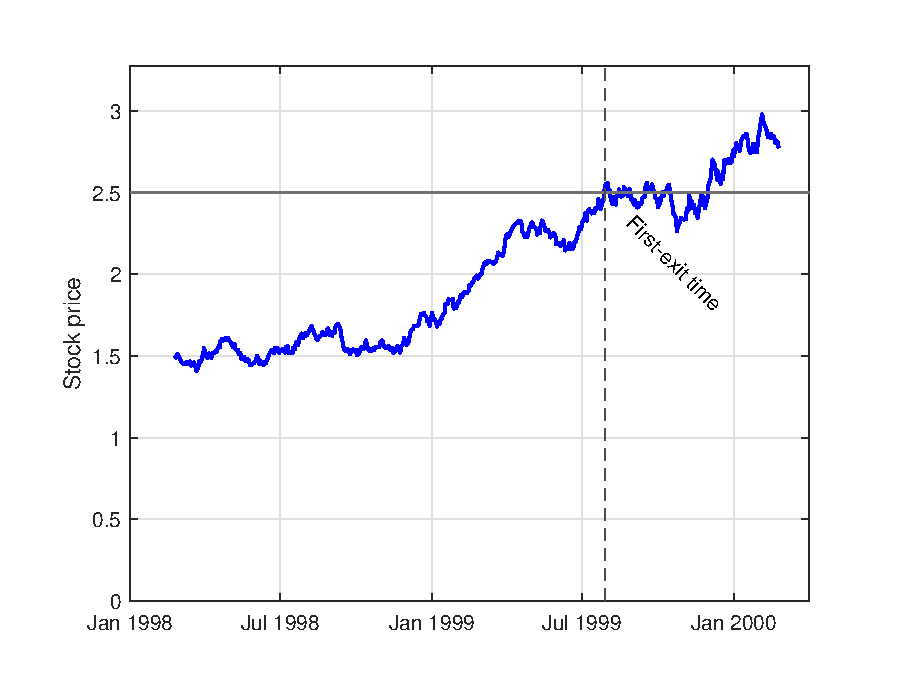
\includegraphics[width=0.65\linewidth]{Imagenes/3_Aleatoriedad/First-exit_Time.eps}
    \caption{First-exit Time}
\end{figure}




\subsubsection{Funciones de distribución acumulada para first-exit times}
Se definde la función $C(y, t; t')$ como la probabilidad de que la variable $y$ salga de la región $\Omega$ antes del tiempo $t'$, habiendo empezado en $y$ en el tiempo $t$. Esta función puede interpretarse como una función de distribución acumulada para first-exit time. 

El objetivo es calcular la probabilidad de que un camino aleatorio abandone una región $\Omega$ antes de un tiempo dado $t'$. Para ello, se tiene que satisfacer el problema de la EDP hacia atrás:
\begin{equation}\label{eq:CumulatFirstExitTime}
    \left\{
    \begin{array}{rlrl}
        \displaystyle\frac{\partial C}{\partial t} + \frac{1}{2} B(y, t)^2 \frac{\partial^2 C}{\partial y^2} + A(y, t) \frac{\partial C}{\partial y} = 0 &\quad& (y,t) \in \Omega\times(0, t') \\[2ex]
        C(y, t; t') = 1 && (y,t) \in \partial\Omega\times(0, t') \\[2ex]
        C(y, t'; t') = 0 && y \in \Omega \\
    \end{array}
    \right\}
\end{equation}




\subsubsection{Tiempos de primer escape esperados (Expected first-exit times)}\label{sec:ExpectedFirstExitTimes}
Una vez calculado~\eqref{eq:CumulatFirstExitTime} es posile calcular el tiempo esperado de primer escape:
\[
    u(y, t) = \int_t^\infty (t' - t) \frac{\partial C}{\partial t'} dt' \overset{\text{partes}}{=} \int_t^\infty 1 - C(y, t; t') dt'
\]
por lo tanto,
\begin{align*}
    \frac{\partial u}{\partial t}  &= \frac{\partial}{\partial t} \left(\int_t^\infty 1 - C(y, t; t') dt' \right) \overset{\text{Leibniz}}{=} -\left(1-C(y, t, t)\right) + \int_t^\infty \frac{\partial}{\partial t}\left(1 - C(y, t; t')\right) dt' \\
    &\overset{\text{\eqref{eq:CumulatFirstExitTime}}}{=} -1 - \int_t^\infty \frac{\partial}{\partial t} C(y, t; t') dt' \\
    \frac{\partial u}{\partial y}  &= \int_t^\infty \frac{\partial}{\partial y}\left(1 - C(y, t; t')\right) dt' = - \int_t^\infty \frac{\partial}{\partial y} C(y, t; t') dt' \\
    \frac{\partial^2 u}{\partial y^2}  &= - \int_t^\infty \frac{\partial^2}{\partial y^2} C(y, t; t') dt' \\
\end{align*}
que volviendo a la EDP~\eqref{eq:CumulatFirstExitTime}:
\begin{align*}
    &\int_t^\infty\frac{\partial C}{\partial t} + \frac{1}{2} B(y, t)^2 \frac{\partial^2 C}{\partial y^2} + A(y, t) \frac{\partial C}{\partial y} dt' = 0 \Rightarrow \\
    &\Rightarrow \int_t^\infty\frac{\partial C}{\partial t} dt' + \frac{1}{2} B(y, t)^2 \int_t^\infty \frac{\partial^2 C}{\partial y^2} dt' + A(y, t) \int_t^\infty \frac{\partial C}{\partial y} dt' = 0 \Rightarrow \\
    &\Rightarrow -1 - \frac{\partial u}{\partial t} - \frac{1}{2} B(y, t)^2 \frac{\partial^2 u}{\partial y^2} - A(y, t) \frac{\partial u}{\partial y} = 0
\end{align*}
por lo que el tiempo esperado de primer escape $u(y, t)$ satisface la EDP:
\[
    \boxed{
        \left\{
        \begin{aligned}
            \frac{\partial u}{\partial t} + \frac{1}{2} B(y, t)^2 \frac{\partial^2 u}{\partial y^2} + A(y, t) \frac{\partial u}{\partial y} = -1\\
            u(y, t) = 0 && y \in \partial\Omega \\
        \end{aligned}
        \right\}
    }
\]
Por ejemplo, si se tiene una EDE independiente del tiempo $A=\mu S, B=\sigma S$, se puede buscar una solución en estado estacionario, es decir, $u(y, t) = u(y)$, que satisface la EDP:
\[
    \frac{1}{2}\sigma^2 S^2 \frac{d^2 u}{dS^2} + \mu S \frac{du}{dS} = -1
\]
con condiciones de contorno $u(S_0) = u(S_1) = 0$. La solución en este caso sería.
\[
    u(S) = \frac{1}{\frac{1}{2}\sigma^2 - \mu} \left( \log(S/S_0) - \frac{1 - (S/S_0)^{1-2\mu/\sigma^2}}{1 - (S_1/S_0)^{1-2\mu/\sigma^2}} \log(S_1/S_0) \right)
\]
















